\section{Approaches}
\label{sec:approach}

In this paper, we introduce a framework named OPTIQ. The framework provides ways to improve data movement performance on the Blue Gene/Q supercomputer. Our framework does so by balancing loads on physical links on the Blue Gene/Q supercomputer.

\subsection{Framework}

Our framework has 3 main components: Path searching algorithms, Schedule and Transport and an extra component depicted in Figure \ref{fig:framework}.

\begin{figure}[!htb]
\vspace{-0.1in}
\centering
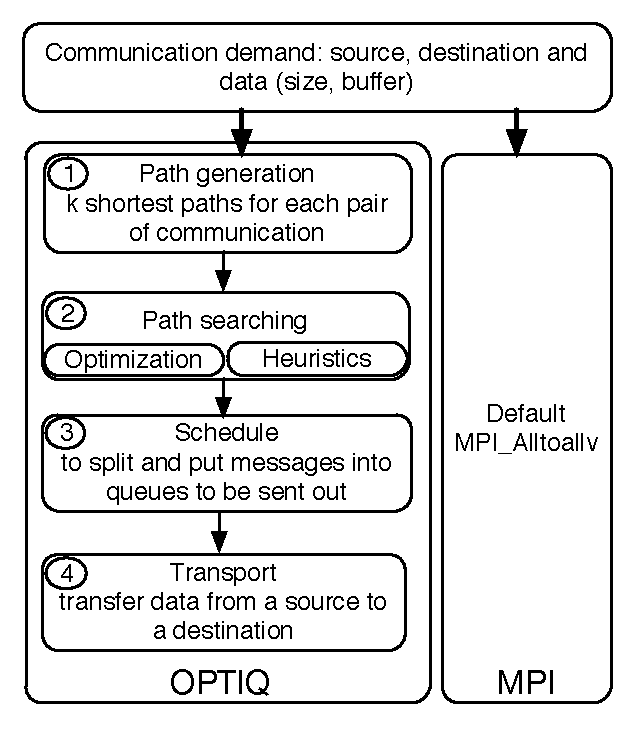
\includegraphics[scale=0.7]{figures/framework.pdf}
\vspace{-0.2in}
\caption{Three components of OPTIQ framework}
\vspace{-0.1in}
\label{fig:framework}
\end{figure}

The functionarity of each component is as following:
\begin{itemize}
\item Path searching: search for path to transfer data from a set of sources to a set of destination. Multiple or single paths can be found using a set of algorithm. User can decide what algorithm to be used or let the framework use a default algorithm.
\item Schedule: Split a buffer data that needed to tranfer into smaller messages and put those messages into a queue of transport layer to be transferred. It also handles incoming messages for itself and for forwardig them to its neighbors on a way to a message final destination.
\item Transport: actually transfer an amount of data from one point to another point in the system.
\item Extra component: To get system specific information such as partition size, topology, coordinates, torus, and to compute neighbors of available nodes given to an application.
\end{itemize}

In the next subsections, we explain in detail our contributions in each component.

\subsection{Path searching layer}
All paths searching algorihtms here are centric algorithms i.e. run at every node in exact oder thus, every node has the same results. The algorithms need some information in advance such as size, topology, torus of the partition, coordinates of all nodes in the partition. The informaition is collected once at the begining. The algorithms, also need to have the pair of source-destination and sometimes the data size to find paths between them.

\subsubsection{Heuristic 1}
In this approach, we search for paths between each pair of source and destination. We explore from all the destination in all possible directions. Whenever we reach a destination, we mark the destination as found to no longer search for it on other explorering paths. In this algorithm, we do not limit exploring paths by any constraints.

\begin{algorithm}
\textbf{Input:} Set of pairs of source-destination (\textit{s$_i$, d$_i$}). Number of nodes \textit{n}. Graph of nodes. \\
\textbf{Output:} Set of paths: one path for a pair of source-destination \\
\\
Init:
    \begin{algorithmic}
	\State queue$<$struct path$>$ \textit{exploring\_paths};
	\State queue$<$struct path$>$ \textit{complete\_paths};
	\State bool \textit{visisted}[\textit{n}][\textit{n}];
	\For {0 $<=$ {\it i}, \textit{j} $<$ \textit{n}} 
	    \State \textit{visited}[{\it i}][{\it j}] = false;
	\EndFor
    \end{algorithmic}
Main:

\begin{algorithmic}
    \Function {Heuristic\_search\_I}{}

    \For {each source \textit{s$_i$}}
	\State check\_and\_add\_new\_path({\it s}$_i$, {\it s}$_i$, null)
    \EndFor

    \While {(\textit{exploring\_path} != empty)}
	\State path \textit{p} = \textit{exploring\_paths}.pop()
	\State get the furthest point {\it u} of {\it p}
	\State check\_and\_add\_new\_path({\it s}$_i$, \textit{u}, {\it p})
    \EndWhile

    \EndFunction
\\
    \Function{check\_and\_add\_new\_path}{int \textit{s$_i$}, int \textit{u}, path {\it op}}
	\For {each neighbor {\it v} of \textit{u}}
	    \If {(!{\it visited}[{\it s$_i$}][{\it v}])}
		\State create an arc \textit{a}$<$\textit{u}, \textit{v}$>$
                \State create a path \textit{np} = {\it op}
	        \State enqueue arc \textit{a} to \textit{np}
	        \State enqueue \textit{np} to \textit{exploring\_paths}
		\If {{\it v} is one of the destinations of \textit{s$_i$}}
		    \State enqueue \textit{np} to \textit{complete\_paths}
                \EndIf
	        \State {\it visited}[\textit{s$_i$}][\textit{v}] = true;
	    \EndIf
	\EndFor
    \EndFunction
\end{algorithmic}

\caption{Heuristic Alg 1: Exploring all paths}
\label{alg:h1}

\end{algorithm}

In the \textbf{Algorithm \ref{alg:h1}}, we start by adding \\

Time complexity: The graph has V vertices and E edges. We have M sources and N destination making K pairs of (source, destinatinon), then the time complexity of the \textbf{Algorithm \ref{alg:h1}} is XXXX.

\subsubsection{Heuristic 2}
This algorithm is an extension from Heuristic 1, while we limit the exploring paths by both the number of hops and minimizing the maximum load. We do so by maintaining a min heap of paths. The comparison function of the heap is based on both the number of hops and maximum load on each path.

\begin{algorithm}

\caption{Heuristic Alg 2: Constraints by number of hops and max load}
\label{alg:h2}
\end{algorithm}

\subsubsection{Heuristic 3}

\begin{algorithm}
\textbf{Input:} Set of pairs of source-destination (\textit{s$_i$, d$_i$}). Number of nodes \textit{n}. Graph of nodes. Number of shortest path \textit{k}\\
\textbf{Output:} Set of paths: \textit{k} paths for a pair of source-destination\\
Init:
    \begin{algorithmic}
        \State queue$<$struct path$>$ \textit{complete\_paths};
    \end{algorithmic}
Main:
\begin{algorithmic}
    \Function {Heuristic\_search\_II}{}
	\For {each pair of source-dest (\textit{s$_i$}, \textit{s$_i$})}
	    \State Use Yen's algorithm to search for \textit{k} shortest paths
	    \State Add \textit{k} shortest paths into \textit{complete\_paths}
	\EndFor
    \EndFunction
\end{algorithmic}

\caption{Heuristic Alg 3: k shortest paths}
\label{alg:h3}

\end{algorithm}

In the \textbf{Algorithm \ref{alg:h3}}, we use Yen's algorithm to search for k shortest paths between \textit{s$_i$, d$_i$}.

\subsubsection{Job-based AMPL model}
In this section we present a formal model written in A Modeling Language for Mathematical Programming (AMPL). The model captures demands of data movement between a set of sources and a set of destinations. The model also capture the graph of physical links of a partition given for the application. The model is presented in Model 1.

We presented the model in AMPL to solve the problem.

\begin{verbatim}
set Nodes;
set Arcs within Nodes cross Nodes;
set Jobs;

param Delay {Arcs} default 0;
param Capacity {Arcs} >= 0 default Infinity;
param Source {Jobs};
param Destination {Jobs} default 0;
param Demand {Jobs} default 0;

var Flow {Jobs, Arcs} >= 0;
var Z >= 0;

var total_flow{(i,j) in Arcs} = 
sum {job in Jobs} Flow[job,i,j];

maximize obj: Z;

subject to

zero_flow {job in Jobs, i in Nodes}:
sum{(i,j) in Arcs} Flow[job,i,j] - 
sum{(j,i) in Arcs} Flow[job,j,i] = 
if (i == Source[job])  then Demand[job]*Z 
else if (i == Destination[job]) then -Demand[job]*Z 
        else 0;

capacity {(i,j) in Arcs}:
total_flow[i,j] <= Capacity[i,j];
\end{verbatim}

Model explanation:
\begin{itemize}
\item sets: we have 3 sets: \textit{Nodes}, \textit{Arcs} and \textit{Jobs}. \textit{JobID}: is the set of transfers from sources to destinations. Each job is represented by a tuple (id, source, destination, demand (total data size to transfer)).
\item params: {\it Delay}: delay on each arc; {\it Capacity}: capacity of each arc; {\it Source}: set of sources; {\it Destination}: set of destinations; {\it Demand}: amount of data to be transferred in each job.
\item vars: \textit{Flow}: total flow of each job on each arc; \textit{Z}: is reversed of total time; \textit{total\_flow} total flow of all jobs going through an arc.
\item objective function: we want to minimize the time or maximize its reversed value i.e. maximize \textit{Z}.
\item constraints(subject to): \textit{zero\_flow}: total flow through a source is total going out of that source, total flow going through a destination is total flow going in that destination, for other nodes that total is 0; \textit{capacity}: total flow on an arc is less than its capacity.
\end{itemize}

\subsubsection{Path-based model}

\subsection{Schedule layer}

As we route data in our own ways, we search for the paths, and we also need to schedule messages transfer. It includes sending local messages, forwarding messages form other sources, receiving data as the intermediate node or the destination node.

Order of messages into sending queue: 3 types of messages: local messages (needed to send), fowarding messages (needed to send), its receiving messages. first come first serve, local messages first. forwa

When there are multiple ranks per node, which one will be choosen to receive data at the next dest (forwarding). Single rank to do or many rank to do, currently every rank executes data transfer.

\subsection{Transport layer}

\subsection{Supported components}

Topology reading, coord, neighbors, torus, size, routing order, graph generated.

Also set of benchmarks, tests.
